% 2026 全国 2 卷 16：三棱锥 A-BCD（E 在棱 BD 上，AE⊥平面 BCD）
% 版面：A 顶部偏左、D 右中、B 左下、C 底部偏右，E 在 BD 上且位于 A 的正下方（故 AE 画成竖直）。
% 虚线（被遮挡）：BD（被 E 分成 B–E、E–D 两段）、AE、EC；其余为可见实线。
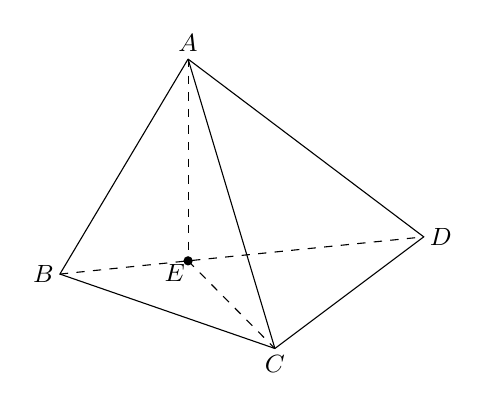
\begin{tikzpicture}[scale=1.05, font=\small]
  \coordinate (A) at (1.55,3.50);
  \coordinate (B) at (0,0.90);
  \coordinate (C) at (2.60,0);
  \coordinate (D) at (4.40,1.35);
  \coordinate (E) at (1.55,1.06);
  % 可见实线
  \draw (A) -- (B) -- (C) -- (D) -- (A);
  \draw (A) -- (C);
  % 被遮挡
  \draw[dashed] (B) -- (E) -- (D);
  \draw[dashed] (A) -- (E);
  \draw[dashed] (E) -- (C);
  \fill (E) circle (1.6pt);
  \node[above,      inner sep=2.5pt] at (A) {$A$};
  \node[left,       inner sep=2pt]   at (B) {$B$};
  \node[below,      inner sep=2.5pt] at (C) {$C$};
  \node[right,      inner sep=2pt]   at (D) {$D$};
  \node[below left, inner sep=1pt]   at (E) {$E$};
\end{tikzpicture}
